\section{Propuesta Boyan}
	\paragraph{}
	Options:
	\begin{itemize}
		\item Ideal case scenario: Global Coverage with lowest possible orbit.
	\item Not so ideal case scenario: Global Coverage with some satellites in a higher orbit acting as a hub.
	\end{itemize}
After reviewing \cite{Wood1998}, \cite{Muri2012}, \cite{Horne2002}, \cite{Wood2001}, \cite{BookchapterinServiceEfficientNetworkInterconnectionviaSatellite2002}, 
\cite{Goodwin1998}, \cite{Sun2015} and \cite{Baumann} my proposal is the next:
\newline

·Use of the \textbf{Manhattan Topology} for our constellation, mixed with a \textit{Walker Delta} or a \textit{Walker Polar} orbits configuration.
\\

%ISL can be very high, with  very high data rates and then, sat to ground can be lower but we can divide it through the network

\textit{"The Manhattan network is the underlying form of the ISL satellite constellation’s
network topology. This is a regular topology named after the regular grid street
pattern established in Manhattan Island, New York. It is a toroidal mesh network with
each node having four unidirectional links: two transmit and two receive
[Maxemchuk87], as shown in figure 2.9.
Manhattan networks have been extensively discussed in computing literature in the
context of parallel computing. The Manhattan network forms the basic topology of the
type (2) constellation. The Manhattan network is also known as a multiaccess mesh or
multimesh network [ToddHahne97]. The form of the Manhattan network with bidirectional
links is known as either the bi-directional Manhattan network, as the HR4-
net [ChungSharAg94], or as the shufflenet.
However, orbital geometry leads to differences from previously discussed Manhattan networks. In fact, the constellation network is a slightly variant form, with bidirectional
ISLs and with two half-twists where the sense of rotation changes due to
each satellite seeing its neighbours swap sides while ‘down’ remains constant as the
satellites reach and pass through their highest latitudes. The topologies of the space
segments of Iridium, Teledesic, and Spaceway NGSO can be considered as variations
on the type of bi-directional Manhattan network shown in figure 2.10."}\cite[p. 32]{Wood2001} \textbf{(en Mendeley)}

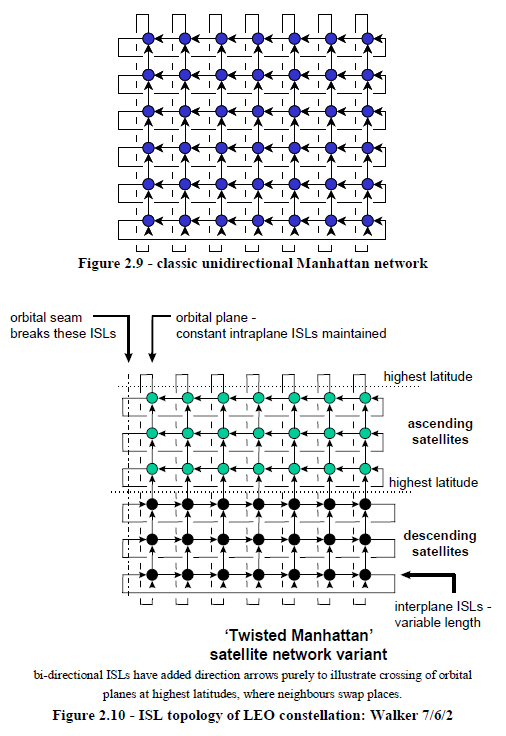
\includegraphics[scale=1]{parts/W_D}
